\chapter{Results and Discussion}\label{chapter:results}
This chapter includes presentation and analysis of the results obtained in this thesis. Section \ref{section:parameter settings} presents results from testing different parameter settings for the genetic algorithm, and briefly discusses each results. Section \ref{section:results} presents the main results obtained when running the different population distributed genetic algorithms. Section \ref{section:discussion} contains a discussion and comparison of the results obtained in section \ref{section:results}.


\section{Parameter settings}\label{section:parameter settings}
Parameter settings are crucial for obtaining good results with the genetic algorithm, therefore, this whole section is devoted to the process. Simulations were run to find the best adult selection method, parent selection method, crossover method, crossover rate and mutation rate for the given problem. Even though it would take much less time and effort to test these values on a toy problem, such as One Max, the decision was made to test them on the real problem. The reason for this is that it is not necessarily true that the parameter values most fit to solve the One Max problem is the same as those most fit to solve the wind farm layout optimization problem. In the wind farm layout optimization problem the relative positions of the turbines are extremely important, this property distinguishes wind farm layout optimization from other problems and could mean that it needs different parameter values than a toy problem with different properties.\\

\noindent It is important to note that even though effort was made to find the right parameter values for the genetic algorithm, it is impossible to obtain the optimal ones. Just imagine trying to test every single value of the continuous parameter crossover rate, just that would be impossible! Therefore, the values that are tested for each parameter are based on the authors previous knowledge and experience with genetic algorithms. \\

\noindent For each simulation presented in this section one parameter were optimized while the others were kept fixed with the values shown in table \ref{table:fixed settings}. The parameters in the table are common for all the genetic algorithm models implemented in this thesis, however, they are only optimized when run on the Master/Slave model. Ideally, they should be optimized for all of the models, but that would not be possible within the time frame of this thesis.\\ 

\begin{table}
\centering
\caption{Values that were kept fixed while one by one were optimized to find the correct settings for the find farm layout optimization problem.}
\label{table:fixed settings}
\begin{tabular}{l|l}
\textbf{Parameter} & \textbf{Value} \\ 
\hline 
Wind scenario & 00.xml \\ 
Evaluator & KusiakLayoutEvaluator \\ 
Population size & 100 \\  
Generations & 100 \\ 
Elitism & true \\  
Flip mutation rate & 0.01 \\ 
Inversion mutation rate & 0.0 \\ 
Interchange mutation rate & 0.0 \\ 
Parent selection & Tournament selection \\ 
Tournament size & 5 \\ 
Epsilon & 0.1 \\  
Crossover method & Uniform crossover \\ 
Crossover rate & 0.9 \\ 
\end{tabular} 
\end{table}

\noindent As can be seen in table \ref{table:fixed settings}, other parameters such as wind scenario, population size, number of generations, whether elitism should be used and mutation rate for interchange mutation and inversion mutation could also be optimized. However, as explained above, the time frame of this thesis prevented the author from running these simulations. These variables are therefore set using the authors previous experience with genetic algorithms. Testing different parameter values on a single wind scenario might lead to values that are tailored for the given scenario and that are not as well suited for some of the other scenarios. However, the author does not believe this to be crucial for the final results. Population size is a value that heavily influence the performance of the genetic algorithm, because greater population size increase the probability of finding the global best solution. When testing parameter values, the population size was kept at 100 for two reasons: First, a population size of 100 is large enough so that many different solutions can be explored. Second, when the population size was kept at 100, the adult selection mechanism overproduction would require 200 evaluations each generation. This doubles the evaluation time, the step that is already the bottleneck of the algorithm. Elitism was set to true for every run, meaning that the best individual of each generation will survive. This decision is based on the authors previous experience with genetic algorithms, where experiments has shown that elitism leads to better results because the best individual is not lost due to coincidences. Three different mutation methods were implemented, but experiments were only run to find the optimal value for the flip mutation rate. Usually, flip mutation is the only mutation methods used with genetic algorithms and it is therefore also used as the main mutation method in this thesis. Inversion mutation and interchange mutation will also be used, but they will be assigned low enough probabilities so that they will not make trouble, but hopefully, lead to occasional, rare jumps from one part of the solution space to another so that the population do not get stuck in a local minima.\\

\noindent In summary, the sub-sections below contain simulations run to find the parameter values most suited for the wind farm layout optimization problem. The resulting parameter values will be used for all 4 genetic algorithm models in section \ref{section:results}. In order to get trustworthy results, each simulation is run 10 times and the plots shown in the subsequent sub-sections are averaged over these 10 simulations. Even though all the models are implemented to run in parallel it takes half a day to run one simulation on an 8 core computer, this is the reason why only the most crucial parameters are optimized and why they are only optimized on the Master/Slave model even thought they will be used by the other models as well.\\

\subsection{Adult Selection}
Figure \ref{plot:adult selection methods} shows the results of running the genetic algorithm with the three different adult selection methods. Sub-figure \ref{plot:full generational replacement}, \ref{plot:generational mixing}, and \ref{plot:overproduction} shows the results for full generational replacement, generational mixing and overproduction respectively. \\

\noindent The results show that full generational replacement ends up with worse fitness than both generational mixing and overproduction, and that overproduction is the method that is able to achieve the best fitness of the three. These results agrees with the authors previous experience. Note that with generational mixing, only the solutions from the new child population that are better than those in the previous adult population are allowed to enter the adult pool. This means that from one generation to another the average fitness of the new adult population can never be worse than the average fitness of the previous adult population. If every new solution generated is worse than those from the previous generation, the previous generation is given another attempt to reproduce and the fitness from one generation to another is left unchanged. However, if one or more of the new solutions are better than those in the previous generation they will be allowed into the adult pool, and the new adult pool will have better fitness than the previous. Full generational replacement does not take this greedy approach. It replaces the entire previous adult population, even though that might lead to worse average fitness form one generation to another. This does not however mean that full generational replacement always obtains worse final results than generational mixing. On this problem however, it seems like the greedy approach taken by generational mixing works well for wind farm layout optimization. Overproduction will, as full generational replacement, replace the entire previous adult pool with new individuals. However, with overproduction, the probability that the new adult population will have better average fitness is much higher since it has twice as many children to choose from. This means that even though it is not guaranteed, it is likely that the new adult population will have higher fitness than the previous one. The results show that overproduction is the most suitable adult selection method for the wind farm layout optimization problem.\\

\begin{figure}[h!]
    \centering
    \begin{subfigure}[b]{0.31\textwidth}
        \includegraphics[width=\textwidth]{images/plots/"adult selection"/"full generational replacement"}
        \caption{}
        \hfill
        \label{plot:full generational replacement}
    \end{subfigure}
    ~
    \begin{subfigure}[b]{0.31\textwidth}
        \includegraphics[width=\textwidth]{images/plots/"adult selection"/"generational mixing"}
        \caption{}
        \hfill
        \label{plot:generational mixing}
    \end{subfigure}
    ~
    \begin{subfigure}[b]{0.31\textwidth}
        \includegraphics[width=\textwidth]{images/plots/"adult selection"/"overproduction"}
        \caption{}
        \hfill
        \label{plot:overproduction}
    \end{subfigure}
    \caption{Adult selection methods: (a) Full generational replacement, (b) generational mixing and (c) overproduction. Each plot shows the averaged results obtained when running each scenario 10 times.}
    \label{plot:adult selection methods}
\end{figure}

\subsection{Parent Selection}
Figure \ref{plot:parent selection} shows the results for running the genetic algorithm with parent selection methods roulette wheel in sub-figure \ref{plot:roulette wheel}, and tournament selection in sub-figures \ref{plot:tournament size 5} - \ref{plot:tournament size 25}. Tournament selection is run with five different values for the variable \textit{tournament size}. Clearly, roulette wheel do not work well for this problem. Roulette wheel assigns each individual a probability of being selected proportional to its fitness, and since there is not a large different in fitness of the different individuals the selection becomes almost random. With tournament selection on the other hand, this problem is taken care of because it finds the best individuals out of those competing, event though there is not much different in their fitness.\\


\noindent As can be seen in the figure, the fitness gets better as the variable \textit{tournament size} increases. However, a larger tournament size than 25 is not tested. The reason for this is that 25 is already a very large tournament size. With 25 \% of the individuals competing in every tournament the population will not have much time to explore different solutions because the best individuals will take over the entire population extremely fast. As can be seen in the figure, a tournament size of 25 is not significantly better than a tournament size of 20, and therefore 20 is chosen as the final tournament size to slow down the take-over time. \\


\noindent As mentioned before, \textit{epsilon} is the probability that the selected individual is selected at random from the adult pool instead of by tournament selection. Figure \ref{plot:epsilon} shows the result for testing the values 5 \%, 10 \%, and 15 \%. As can be seen in the figure, varying epsilon does not have a significant impact on the fitness on the wind farm layout optimization problem.\\


\begin{figure}[h!]
    \centering
    \begin{subfigure}[b]{0.31\textwidth}
        \includegraphics[width=\textwidth]{images/plots/"parent selection"/"roulette wheel"}
        \caption{}
        \hfill
        \label{plot:roulette wheel}
    \end{subfigure}
    ~
    \begin{subfigure}[b]{0.31\textwidth}
        \includegraphics[width=\textwidth]{images/plots/"parent selection"/"tournament size 5"}
        \caption{}
        \hfill
        \label{plot:tournament size 5}
    \end{subfigure}
    ~
       \begin{subfigure}[b]{0.31\textwidth}
        \includegraphics[width=\textwidth]{images/plots/"parent selection"/"tournament size 10"}
        \caption{}
        \hfill
        \label{plot:tournament size 10}
    \end{subfigure}
    ~
       \begin{subfigure}[b]{0.31\textwidth}
        \includegraphics[width=\textwidth]{images/plots/"parent selection"/"tournament size 15"}
        \caption{}
        \hfill
        \label{plot:tournament size 15}
    \end{subfigure}
    ~
       \begin{subfigure}[b]{0.31\textwidth}
        \includegraphics[width=\textwidth]{images/plots/"parent selection"/"tournament size 20"}
        \caption{}
        \hfill
        \label{plot:tournament size 20}
    \end{subfigure}
    ~
    \begin{subfigure}[b]{0.31\textwidth}
        \includegraphics[width=\textwidth]{images/plots/"parent selection"/"tournament size 25"}
        \caption{}
        \hfill
        \label{plot:tournament size 25}
    \end{subfigure}
    \caption{Parent selection methods: (a) Roulette wheel, (b) tournament selection, tournament size 5 (c) tournament selection, tournament size 10, (d) tournament selection, tournament size 15, (e) tournament selection, tournaments size 20, and (f) tournament selection, tournament size 25. Each result is an average over 10 runs.}
    \label{plot:parent selection}
\end{figure}


\begin{figure}[h!]
    \centering
    \begin{subfigure}[b]{0.31\textwidth}
        \includegraphics[width=\textwidth]{images/plots/epsilon/"tournament size 20"/"epsilon 0,05"}
        \caption{}
        \hfill
        \label{plot:epsilon 0.05}
    \end{subfigure}
    ~
    \begin{subfigure}[b]{0.31\textwidth}
        \includegraphics[width=\textwidth]{images/plots/epsilon/"tournament size 20"/"epsilon 0,10"}
        \caption{}
        \hfill
        \label{plot:epsilon 0.10}
    \end{subfigure}
    ~
    \begin{subfigure}[b]{0.31\textwidth}
        \includegraphics[width=\textwidth]{images/plots/epsilon/"tournament size 20"/"epsilon 0,15"}
        \caption{}
        \hfill
        \label{plot:epsilon 0.15}
    \end{subfigure}
    \caption{Different epsilon values: (a) Epsilon 0.05, (b) epsilon 0.10, and (c) epsilon 0.15. The tournament size was kept fixed at 20 since that was proven to give the best results. Each plot is an average over 10 runs.}
    \label{plot:epsilon}
\end{figure}


\subsection{Crossover Methods}
Figure \ref{plot:crossover methods} show the results when running the genetic algorithm with single point crossover, two point crossover, and uniform crossover as can be seen in sub figures \ref{plot:single point crossover}, \ref{plot:two point crossover}, and \ref{plot:uniform crossover} respectively. The experiment show that no crossover method is significantly better than the others in solving the wind farm layout optimization problem. This result is unexpected. Intuitively, one would expect uniform crossover to perform worse because it mixes up the relative positions of the wind turbines more than single point crossover and two point crossover. However, the results contradicts this hypothesis. \\


\begin{figure}[h!]
    \centering
    \begin{subfigure}[b]{0.31\textwidth}
        \includegraphics[width=\textwidth]{images/plots/"crossover method"/"single point crossover"}
        \caption{}
        \hfill
        \label{plot:single point crossover}
    \end{subfigure}
    ~
    \begin{subfigure}[b]{0.31\textwidth}
        \includegraphics[width=\textwidth]{images/plots/"crossover method"/"two point crossover"}
        \caption{}
        \hfill
        \label{plot:two point crossover}
    \end{subfigure}
    ~
    \begin{subfigure}[b]{0.31\textwidth}
        \includegraphics[width=\textwidth]{images/plots/"crossover method"/"uniform crossover"}
        \caption{}
        \hfill
        \label{plot:uniform crossover}
    \end{subfigure}
    \caption{Crossover methods averaged over 10 runs: (a) Single point crossover, (b) two point crossover and (c) uniform crossover.}
    \label{plot:crossover methods}
\end{figure}


\subsection{Crossover Rate}
Figure \ref{plot:crossover rates} displays the results of running the genetic algorithm with different crossover rates. As can be seen in the figure, the crossover rate do not have a large impact on the fitness for this problem. A crossover rate below 0.4 gives slightly worst fitness than a crossover rate above 0.6. However, it is not obvious which crossover rate is best out of those presented in sub-figures \ref{plot:crossover rate 0.6}, \ref{plot:crossover rate 0.8}, and \ref{plot:crossover rate 1.0}. The differences in the results obtained when running the algorithm with these crossover rates are not significant, and it can not be stated that one is better than the others based on these results. It can only be stated that a crossover rate above 0.6 should be used. \\


\begin{figure}[h!]
    \centering
    \begin{subfigure}[b]{0.31\textwidth}
        \includegraphics[width=\textwidth]{images/plots/"crossover rate"/"crossover rate 0,0"}
        \caption{}
        \hfill
        \label{plot:crossover rate 0.0}
    \end{subfigure}
    ~
    \begin{subfigure}[b]{0.31\textwidth}
        \includegraphics[width=\textwidth]{images/plots/"crossover rate"/"crossover rate 0,2"}
        \caption{}
        \hfill
        \label{plot:crossover rate 0.2}
    \end{subfigure}
    ~
       \begin{subfigure}[b]{0.31\textwidth}
        \includegraphics[width=\textwidth]{images/plots/"crossover rate"/"crossover rate 0,4"}
        \caption{}
        \hfill
        \label{plot:crossover rate 0.4}
    \end{subfigure}
    ~
       \begin{subfigure}[b]{0.31\textwidth}
        \includegraphics[width=\textwidth]{images/plots/"crossover rate"/"crossover rate 0,6"}
        \caption{}
        \hfill
        \label{plot:crossover rate 0.6}
    \end{subfigure}
    ~
       \begin{subfigure}[b]{0.31\textwidth}
        \includegraphics[width=\textwidth]{images/plots/"crossover rate"/"crossover rate 0,8"}
        \caption{}
        \hfill
        \label{plot:crossover rate 0.8}
    \end{subfigure}
    ~
    \begin{subfigure}[b]{0.31\textwidth}
        \includegraphics[width=\textwidth]{images/plots/"crossover rate"/"crossover rate 1,0"}
        \caption{}
        \hfill
        \label{plot:crossover rate 1.0}
    \end{subfigure}
    \caption{Crossover rates average over 10 runs: (a) Crossover rate 0.0, (b) crossover rate 0.2, (c) crossover rate 0.4, (d) crossover rate 0.6, (e) crossover rate 0.8, and (f) crossover rate 1.0.}
    \label{plot:crossover rates}
\end{figure}


\subsection{Mutation Rate}
In figure \ref{plot:mutation rate}, the effect of varying the mutation rate can be seen. As the figure shows, if the mutation rate is very low as shown in sub-figure \ref{plot:mutation rate 0.0001}, the population is clearly not able to find a good solution. Mutation means adding or removing a turbine. As sub-figure \ref{plot:mutation rate 0.0001} show, with a mutation rate that is too low the genetic algorithm will not be able to add or remove enough turbines and therefore the population ends up in a local minima. On the other hand, when the mutation rate gets too high, as shown in sub-figure \ref{plot:mutation rate 0.01}, the population is able to explore many different solutions something that increases its chance of finding the global minima. However, since mutation is performed too frequently, it is not able to stay there even if it finds the global optimal solution. These results show that mutation rate largely impacts the fitness, and that a mutation rate of 0.001 clearly gives the best results.


\begin{figure}[h!]
    \centering
      \begin{subfigure}[b]{0.31\textwidth}
        \includegraphics[width=\textwidth]{images/plots/"mutation rate"/"mutation rate 0,0001"}
        \caption{}
        \hfill
        \label{plot:mutation rate 0.0001}
    \end{subfigure}
    ~
      \begin{subfigure}[b]{0.31\textwidth}
        \includegraphics[width=\textwidth]{images/plots/"mutation rate"/"mutation rate 0,0005"}
        \caption{}
        \hfill
        \label{plot:mutation rate 0.0005}
    \end{subfigure}
    ~
    \begin{subfigure}[b]{0.31\textwidth}
        \includegraphics[width=\textwidth]{images/plots/"mutation rate"/"mutation rate 0,001"}
        \caption{}
        \hfill
        \label{plot:mutation rate 0.001}
    \end{subfigure}
    ~
    \begin{subfigure}[b]{0.31\textwidth}
        \includegraphics[width=\textwidth]{images/plots/"mutation rate"/"mutation rate 0,005"}
        \caption{}
        \hfill
        \label{plot:mutation rate 0.005}
    \end{subfigure}
    ~
    \begin{subfigure}[b]{0.31\textwidth}
        \includegraphics[width=\textwidth]{images/plots/"mutation rate"/"mutation rate 0,01"}
        \caption{}
        \hfill
        \label{plot:mutation rate 0.01}
    \end{subfigure}
    \caption{Mutation rate averaged over 10 runs: (a) Mutation rate 0.0001, (b) mutation rate 0.0005 and (c) mutation rate 0.001, (d) mutation rate 0.005 and (e) mutation rate 0.01s.}
    \label{plot:mutation rate}
\end{figure}


\section{Results}\label{section:results}


\subsection{Final Parameter Values}
This sub-section gives an overview of the final parameter values that will be used in the subsequent sub-section when running the different models. Table \ref{table:final parameter settings master slave model} provides an overview of the parameter values that will be used when running the Master/Slave model. The adult selection method, parent selection method, parent selection parameters, crossover method, crossover rate and mutation rate are those that was proven to work best for the Master/Slave model in section \ref{section:parameter settings}. As table \ref{table:final parameter settings master slave model} show, the population size was set to 100 and the number of generations to 200. A population size of 100 is quite small, but since overproduction is the selected adult selection method, a population size of 100 leads to evaluation of 200 individuals for each generation. Since evaluation is the bottleneck for wind farm layout optimization, a larger population size would not be possible to evaluate for 200 generations within the time limits of this thesis. A possibility could be to pick a larger population size and a smaller number of generations, but since the objective of this thesis is to explore population distributed genetic algorithms a large number of generations is crucial. Population distributed genetic algorithms need more time to find good solutions because they spend more time than simple genetic algorithms on exploring different parts of the search space.\\

\begin{table}[h!]
\centering
\caption{Parameter values used for the Master/Slave model.}
\label{table:final parameter settings master slave model}
\begin{tabular}{l|l}
\textbf{Parameter} & \textbf{Value} \\ 
\hline 
Population size & 100 \\  
Generations & 200 \\ 
Crossover method & Single point crossover \\ 
Crossover rate & 0.9 \\ 
Elitism & True \\ 
Flip mutation rate & 0.001 \\ 
Inversion mutation rate & 0.000001 \\ 
Interchange mutation rate & 0.000001 \\ 
Adult selection mechanism & Overproduction \\ 
Parent selection mechanism & Tournament selection \\ 
Tournament size & 20\% of population size\\ 
Epsilon & 0.1 \\ 
\end{tabular} 
\end{table}

\noindent The parameter values in table \ref{table:final parameter settings master slave model} will also be used for all of the population distributed models if not otherwise stated. Table \ref{table:final parameter settings island model} contains the additional parameter values used by the Island model, and those parameters from table \ref{table:final parameter settings master slave model} that have new values for the Island model. The parameter \textit{deme size}, the number of individuals on each Island, is set to 26 resulting in a total population size of 104, not 100 as in table \ref{table:final parameter settings master slave model}. The reason behind this is that the implementation requires a population size of even numbers on each Island, this is not a problem since a few additional individuals will not be enough to impact the final results. The parameter \textit{migration rate} was set to 2, meaning that only 7 \% of the individuals on an Island are replaced by new individuals each migration. This number was set to be low so that the new individuals would not be able to take over the new population too fast. The parameter \textit{deme count} is set to 4 and the topology is circular as presented in figure \ref{figure:topology island model} in chapter \ref{chapter:methodology}. In order to let the populations on the different Islands explore different parts of the search space 20 generations are run between each migration. Migration is performed 10 times so that the total number of generations becomes 200 as for the Master/Slave model.\\

\begin{table}[h!]
\centering
\caption{Parameter values used for the Island model.}
\label{table:final parameter settings island model}
\begin{tabular}{l|l}
\textbf{Parameter} & \textbf{Value} \\ 
\hline 
Deme size & 26 \\
Total population size & 104 \\  
Deme count & 4 \\
Migration rate & 2 \\
Number of migrations & 10 \\ 
Migration interval & 20 \\
Topology & Circular (figure \ref{figure:topology island model}) \\
\end{tabular}
\end{table}

\noindent As can be seen in table \ref{table:final parameter settings pool model}, the Cellular model is run with population size of 225. At a first glance this might seem like an odd decision since the models above has a population size of about 100 individuals, but the reason is simple. For the Master/Slave model, and Island model overproduction is used as the adult selection technique because it was proven the best technique in section \ref{section:parameter settings}. For the Cellular model however, it does not make sense to use overproduction because of the way the grid is updated. Each new individual is generated to occupy a particular spot in the grid, because it has its own area for which its parents can be chosen from. Since each new individual is mapped to one position in the grid, overproduction does not make sense to use and it is therefore not used for the Cellular model. Because of this, the population size is set to approximately 200 individuals, so that the Cellular model performs the same number of evaluations as the other models each generation. The reason why the population size is 225 and not 200 is because a quadratic grid is used to distribute the production and 225 is equal to 15$^{2}$. As explained in the methodology chapter, the topology used is a simple square containing nine individuals. The individual in the middle square can only be replaced by individuals generated by recombining individuals within the square grid. The decision to make the neighborhood this small is that it will give different solutions the opportunity to dominate different areas of the grid, giving the algorithm the time to explore.\\


\begin{table}
\centering
\caption{Parameter values used for the Cellular model.}
\label{table:final parameter settings cellular model}
\begin{tabular}{l|l}
\textbf{Parameter} & \textbf{Value} \\ 
\hline 
Population size & 225 \\
Topology & Square (figure \ref{figure:cellular model topology}) \\  
\end{tabular}
\end{table}

\noindent Table \ref{table:final parameter settings pool model} shows the parameter values used by the Pool model that differs from those in table \ref{table:final parameter settings master slave model}. The population size is set to 200 so that 200 evaluations are performed for each of the 200 generations. As for the Cellular model, the individuals of the Pool model occupy specific positions. Child generation consist of producing one new individual for each position that a worker is responsible for. If overproduction was used, it would be no clear mapping between new child individuals and the old individuals of the worker because twice as many individuals as position would be generated, this does not make sense for the Pool model. Because of this a population size of 200 individuals where used so that 200 evaluations are performed for each generation as for the other models.\\

\begin{table}[h!]
\centering
\caption{Parameter values used for the Pool model.}
\label{table:final parameter settings pool model}
\begin{tabular}{l|l}
\textbf{Parameter} & \textbf{Value} \\ 
\hline 
Population size & 200 \\  
Number of workers & 4 \\ 
\end{tabular}
\end{table}

\noindent In summary, in order to make the comparison as fair as possible, the parameter values of each models is set so that approximately 200 individuals are evaluated for each of the 200 generations. This ensures that every model gets approximately the same processor time.\\


\subsection{Performance Metrics}\label{subsection:performance metrics}
\noindent Each of the 4 genetic algorithm models are tested on 4 wind scenarios. The wind scenarios are provided by GECCO 2016 and can be seen in table \ref{table:scenario properties}. As can be seen, the first two scenarios are without obstacles, while the two last scenarios are with obstacles.\\

\begin{table}[h!]
\centering
\caption{Test scenarios provided by GECCO 2016.}
\label{table:scenario properties}
\begin{tabular}{l|l}
\textbf{Scenario Name} & \textbf{Obstacles} \\
\hline
00.xml            & No obstacles. \\
05.xml            & No obstacles. \\
obs00.xml         & Obstacles. \\
obs05.xml         & Obstacles. \\
\end{tabular}
\end{table}

\noindent The performance of the 4 models on each of the four scenarios are measured using the performance metrics shown in table \ref{table:performance metrics}. The first performance metric is the results of the fitness function presented in chapter \ref{chapter:methodology}. The efficiency is a measure of how much energy the given layout is able to produce out of the power the layout would have been able to produce had there been no wake effect, as shown in equation \ref{equation:efficiency}

\begin{equation}
\textrm{efficiency} = \frac{\textrm{yearly power output}}{\textrm{wake free yearly power output}}.
\label{equation:efficiency}
\end{equation}

\noindent The performance metrics cost and power represent the cost and power part of the fitness function. Figure \ref{figure:performance metrics cost and power}, shows which parts of the fitness function presented in chapter \ref{chapter:methodology} that represents cost and which represents power. The last metric, number of turbines, is intuitively the total number of turbines in the layout.\\ 

\begin{figure}[h!]
\begin{center}
\includegraphics[scale=0.5]{images/"performance metrics"}
\caption{A screen shot of the fitness function presented in chapter \ref{chapter:methodology} where the cost and power metrics are shown.}
\label{figure:performance metrics cost and power}
\end{center}
\end{figure}

\begin{table}[h!]
\centering
\caption{For each scenario, results are measured in these measurements.}
\label{table:performance metrics}
\centering
\begin{tabular}{l|l}
\textbf{Results measured}   & \textbf{Description} \\
\hline
Fitness                     & Fitness of the best individual \\
Efficiency                  & Amount of power produced out of maximum \\
Cost                        & Total cost (USD)\\
Power                       & Yearly power output (kWh) \\
Number of turbines          & Total number of turbines
\end{tabular}
\end{table}

\noindent In chapter \ref{chapter:background}, one of the resulting layout from \citep{Grady} was shown as an example layout. In this thesis, the resulting layout will be to large to include. Additionally, with the realistic wind scenarios used, the wind turbines will be scattered around in the grid in a way that would not make sense to look at. The performance metrics above on the other hand, gives a much more clear understanding of the performance of the models and are the metrics that will be used to present the results.\\


\subsection{Results Scenario 00}
The results when all the models were run on scenario 00.xml is shown in figure \ref{plot:scenario 00}. The fitness plot is shown in sub-figure \ref{plot:fitness plot scenario 00}. The Master/Slave model is able to get the best fitness, the Pool model comes in second, quite close to the Master/Slave model, the Island model comes in third, and the Cellular model comes in forth, clearly not able to keep up with the other models.\\ 


\noindent Sub-figure \ref{plot:efficiency plot scenario 00} shows the performance of the different models in terms of efficiency. Efficiency is a very interesting measure, since it shows the models' ability to live up to their potential. As will be discussed below, the Master/Slave model and Pool model end up with a different number of turbines. Interestingly, within their chosen number of turbines, both models are able to obtain almost the same efficiency, showing that they are both good at optimizing turbine positions.\\


\noindent As shown in sub-figures \ref{plot:cost plot scenario 00} and \ref{plot:turbines plot scenario 00}, the plots for cost and number of turbines have identical shape. This makes sense off course since the cost increase and decrease with the number of turbines. The plots show that the Master/Slave model end up with a larger number of turbines than the other models, which all end up with the same number of turbines. The Master/Slave model, the Pool model and the Cellular model all decide on the number of turbines before having evolved for 20 generations, while the Island model is able to explore different solutions until around generation 50, when it stabilized on the same solution as the Pool- and Cellular model. The Island model cost plot has a different shape than the other plots. While the other models slowly go from one solution to another, the Island model jumps from one part of the solution space to another. These observations make sense, because, these jumps occur at generation 20 and 40, the generations where the first and second migration takes place. 

Between generation 20 and 40, the Island model explores a solution with the same number of turbines as the Master/Slave model, a solution that could be the global minima. However, the Island model is not able to stay in this minima, because it observes that jumping to a solution with fewer turbines seems more promising. If the migration interval had been longer than 20 generations, the Island model might have been able to optimize turbine positions in the global minima so that it would discover the true potential of the solution before leaving it for a sub-optimal solution.\\


\noindent The performance of the different models can be viewed in terms of power in sub-figure \ref{plot:power plot scenario 00}. Power is also closely related to the number of turbines. Clearly a solution with more turbines leads to higher energy output. However, as the Island model power plot shows, solutions with high power production might not be prioritized because the cost becomes too high so that the total fitness becomes worse. After the models have stabilized on a particular number of turbines, the power is slowly increasing. This is because the turbines are slowly moved into positions with less wake loss. \\


\noindent In summary, the optimization can be viewed as consisting of two phases. The first phase is the search for the optimal number of turbines, while the second phase consist of moving turbines around in order to reduce wake loss. The Island model stays in phase one longer than the other models. Still, the Master/Slave model is the only model able to find what could be the global optimal solution in terms of the number of turbines. \\

\begin{figure}[h!]
    \centering
      \begin{subfigure}[b]{0.45\textwidth}
        \includegraphics[width=\textwidth]{images/plots/Plots/"scenario 00"/"best"}
        \caption{Fitness}
        \hfill
        \label{plot:fitness plot scenario 00}
    \end{subfigure}
    ~
      \begin{subfigure}[b]{0.45\textwidth}
        \includegraphics[width=\textwidth]{images/plots/Plots/"scenario 00"/"efficiency"}
        \caption{Efficiency}
        \hfill
        \label{plot:efficiency plot scenario 00}
    \end{subfigure}
    ~
    \begin{subfigure}[b]{0.45\textwidth}
        \includegraphics[width=\textwidth]{images/plots/Plots/"scenario 00"/"cost"}
        \caption{Cost}
        \hfill
        \label{plot:cost plot scenario 00}
    \end{subfigure}
    ~
    \begin{subfigure}[b]{0.45\textwidth}
        \includegraphics[width=\textwidth]{images/plots/Plots/"scenario 00"/"power"}
        \caption{Power}
        \hfill
        \label{plot:power plot scenario 00}
    \end{subfigure}
    ~
    \begin{subfigure}[b]{0.45\textwidth}
        \includegraphics[width=\textwidth]{images/plots/Plots/"scenario 00"/"turbines"}
        \caption{Turbies}
        \hfill
        \label{plot:turbines plot scenario 00}
    \end{subfigure}
    \caption{Scenario 00.xml averaged over 10 runs: (a) Fitness plot, (b) efficiency plot, (c) cost plot, (d) power plot, and (e) number of turbines.}
    \label{plot:scenario 00}
\end{figure}


\subsection{Results Scenario 05}
The results for running the different models on scenario 05.xml is shown in figure \ref{plot:scenario 05}. The fitness plot is shown in sub-figure \ref{plot:fitness plot scenario 05}. As for scenario 00.xml, the Master/Slave model obtains the best fitness closely followed by the Pool model. The Island model comes in third again, and the Cellular model is not able to keep up with the other models on this scenario either. After 200 generations the Cellular model has a fitness which each of the other models had beaten already at generation 10.\\


\noindent The efficiency plot is shown in sub-figure \ref{plot:efficiency plot scenario 05}. As before, the Master/Slave model and Pool model is able to find a solution with approximately the same efficiency. The Island model is a few steps behind, while the efficiency of the Cellular model is increasing extremely slowly. \\


\noindent Sub-figures \ref{plot:cost plot scenario 05} and \ref{plot:turbines plot scenario 05} shows cost plot and number of turbines plot respectively. As can be seen, the Master/Slave model and Pool model does not explore different number of turbines, they both stabilize on a given number after less than 10 generations. The Cellular model explores for about 15-20 generations before it decide on the number of turbines. From the sub-figures it looks like the Island model explores for a little less than 50 generations, but if one takes a closer look, it actually does a small jump to a solution with fewer turbines at about generation 80. However, it is not able to stay in this solutions for longer than about 5 generations. As for scenario 00.xml, the Master/Slave model ends up with a higher number of turbines than the other 3 models. It seems like the Master/Slave model has found the global minima, or at least a better local minima than the other models, something that might explain why the Pool model is not able to get a fitness as good as the Master/Slave model.\\


\noindent Power is closely related to the number of turbines, and as can be seen in sub-figure \ref{plot:power plot scenario 05}, the Master/Slave model finds the solution that is able to produce most energy. The Pool Model and Island model both end up with the same number of turbines, and as can be seen the amount of power that they are able to produce is similar. The Pool model produces a little more power because it is able to find better positions for the turbines as can be seen since it beats the Pool model in fitness and efficiency. \\


\begin{figure}[h!]
    \centering
      \begin{subfigure}[b]{0.45\textwidth}
        \includegraphics[width=\textwidth]{images/plots/Plots/"scenario 05"/"best"}
        \caption{Fitness}
        \hfill
        \label{plot:fitness plot scenario 05}
    \end{subfigure}
    ~
      \begin{subfigure}[b]{0.45\textwidth}
        \includegraphics[width=\textwidth]{images/plots/Plots/"scenario 05"/"efficiency"}
        \caption{Efficiency}
        \hfill
        \label{plot:efficiency plot scenario 05}
    \end{subfigure}
    ~
    \begin{subfigure}[b]{0.45\textwidth}
        \includegraphics[width=\textwidth]{images/plots/Plots/"scenario 05"/"cost"}
        \caption{Cost}
        \hfill
        \label{plot:cost plot scenario 05}
    \end{subfigure}
    ~
    \begin{subfigure}[b]{0.45\textwidth}
        \includegraphics[width=\textwidth]{images/plots/Plots/"scenario 05"/"power"}
        \caption{Power}
        \hfill
        \label{plot:power plot scenario 05}
    \end{subfigure}
    ~
    \begin{subfigure}[b]{0.45\textwidth}
        \includegraphics[width=\textwidth]{images/plots/Plots/"scenario 05"/"turbines"}
        \caption{Turbies}
        \hfill
        \label{plot:turbines plot scenario 05}
    \end{subfigure}
    \caption{Scenario 05.xml averaged over 10 runs: (a) Fitness plot, (b) efficiency plot, (c) cost plot, (d) power plot, and (e) number of turbines.}
    \label{plot:scenario 05}
\end{figure}


\subsection{Results Scenario obs00.xml}
Figure \ref{plot:scenario obs 00} shows the results obtained when running the model on scenario obs00.xml. As for scenairo 00.xml and 05.xml, the Master/Slave model obtains the best fitness, the Pool model the second best, the Island model third best and the Cellular model the fourth best, as can be seen in sub-figure \ref{plot:fitness plot scenario obs 00}.\\


\noindent As for efficiency, the results are similar as those observed for scenario 00.xml and scenario 05.xml as can be seen in sub-figure \ref{plot:efficiency plot scenario obs 00}. Both the Pool model and Island model are able to optimize their solutions so that they produce more than 84.5 \% of the wake free energy. The Island model however, is only able to produce just above 83.5 \% of the wake free energy.\\


\noindent As shown in sub-figures \ref{plot:cost plot scenario obs 00} and \ref{plot:turbines plot scenario obs 00} the Island- and Cellular model end up with the same number of turbines, while the Master/Slave- and Pool model end up with different number of turbines. The Island- and Cellular model ends up at the solution with the highest number of turbines and the Pool models finds the solution with fewest turbines. This explains why the Island model scored so badly on efficiency, it finds out that adding turbines leads to higher power production and therefore better fitness and therefore it ends up in a sub-optimal solution. \\


\noindent The Island model finds the solutions which produces most power, a reasonable result since no other model ends up with more turbines. However, the Island model is closely followed by the Master/Slave model even though it finds a solution with fewer turbines. This shows that the Master/Slave model is way better at optimizing the turbine positions. On problematic observation is that the Cellular model ends up with a solution that produces less power than all the other models even thought it ends up with a solution with the same number of turbines as the Island model. This results show that the Cellular model is not able to find a solution that position the turbines well within 200 generations. \\


\begin{figure}[h!]
    \centering
      \begin{subfigure}[b]{0.45\textwidth}
        \includegraphics[width=\textwidth]{images/plots/Plots/"scenario obs 00"/best}
        \caption{Fitness}
        \hfill
        \label{plot:fitness plot scenario obs 00}
    \end{subfigure}
    ~
      \begin{subfigure}[b]{0.45\textwidth}
        \includegraphics[width=\textwidth]{images/plots/Plots/"scenario obs 00"/efficiency}
        \caption{Efficiency}
        \hfill
        \label{plot:efficiency plot scenario obs 00}
    \end{subfigure}
    ~
    \begin{subfigure}[b]{0.45\textwidth}
        \includegraphics[width=\textwidth]{images/plots/Plots/"scenario obs 00"/cost}
        \caption{Cost}
        \hfill
        \label{plot:cost plot scenario obs 00}
    \end{subfigure}
    ~
    \begin{subfigure}[b]{0.45\textwidth}
        \includegraphics[width=\textwidth]{images/plots/Plots/"scenario obs 00"/power}
        \caption{Power}
        \hfill
        \label{plot:power plot scenario obs 00}
    \end{subfigure}
    ~
    \begin{subfigure}[b]{0.45\textwidth}
        \includegraphics[width=\textwidth]{images/plots/Plots/"scenario obs 00"/turbines}
        \caption{Turbies}
        \hfill
        \label{plot:turbines plot scenario obs 00}
    \end{subfigure}
    \caption{Scenario obs00.xml averaged over 10 runs: (a) Fitness plot, (b) efficiency plot, (c) cost plot, (d) power plot, and (e) number of turbines.}
    \label{plot:scenario obs 00}
\end{figure}


\subsection{Results Scenario obs05.xml}


\noindent Figure \ref{plot:scenario obs 05} shows the results from scenario obs05.xml averaged over 10 runs. Fitness is shown in sub-figure \ref{plot:fitness plot scenario 05}. As can be seen, the results are similar to the results for the other 3 scenarios.\\


\noindent Since the result is similar to those observed before, they will not be discussed in details here, however one interesting observation has been made: In sub-figures \ref{plot:cost plot scenario obs 05} and \ref{plot:turbines plot scenario obs 05} it can be observed that every model end up in solutions with a different number of turbines. These results shows the complexity of the problem by showing how easy it is to end up in a local minima. Because, even thought the global minima is not known it is known that at least 3 of the models are stuck in a local minima.  \\


\begin{figure}[h!]
    \centering
      \begin{subfigure}[b]{0.45\textwidth}
        \includegraphics[width=\textwidth]{images/plots/Plots/"scenario obs 05"/best}
        \caption{Fitness}
        \hfill
        \label{plot:fitness plot scenario obs 05}
    \end{subfigure}
    ~
      \begin{subfigure}[b]{0.45\textwidth}
        \includegraphics[width=\textwidth]{images/plots/Plots/"scenario obs 05"/efficiency}
        \caption{Efficiency}
        \hfill
        \label{plot:efficiency plot scenario obs 05}
    \end{subfigure}
    ~
    \begin{subfigure}[b]{0.45\textwidth}
        \includegraphics[width=\textwidth]{images/plots/Plots/"scenario obs 05"/cost}
        \caption{Cost}
        \hfill
        \label{plot:cost plot scenario obs 05}
    \end{subfigure}
    ~
    \begin{subfigure}[b]{0.45\textwidth}
        \includegraphics[width=\textwidth]{images/plots/Plots/"scenario obs 05"/power}
        \caption{Power}
        \hfill
        \label{plot:power plot scenario obs 05}
    \end{subfigure}
    ~
    \begin{subfigure}[b]{0.45\textwidth}
        \includegraphics[width=\textwidth]{images/plots/Plots/"scenario obs 05"/turbines}
        \caption{Turbies}
        \hfill
        \label{plot:turbines plot scenario obs 05}
    \end{subfigure}
    \caption{Scenario obs05.xml averaged over 10 runs: (a) Fitness plot, (b) efficiency plot, (c) cost plot, (d) power plot, and (e) number of turbines.}
    \label{plot:scenario obs 05}
\end{figure}


\section{Discussion}\label{section:discussion}
\noindent In the previous section it was shown that the non-population distributed Master/Slave model consistently was able to evolve layouts with better fitness than the 3 population distributed models. The Pool model came in second, the Island model came in third and the Cellular model came in fourth and last. There can be many reasons for this, and they will all be discussed in this section. The main results are listed below.\\

\begin{itemize}
\item The non-population distributed Master/Slave model was the model able to obtain the best results. 
\item The Pool model obtained the second best results.
\item The Island model obtained the third best results.
\item The Cellular model obtained the forth best results.
\end{itemize}

\noindent As mentioned earlier, wind farm layout optimization is extremely hard, if not impossible, to solve analytically. The solution space is simply too huge for any computer to evaluate every possible wind farm layout to find the best layout. For a wind farm with only 500 legal turbine positions, 2$^{100}$ different layouts exists! With a solution space this large, it is very unlikely that a genetic algorithm is able to find the global optimal solution. As the results show, the Master/Slave model only spend less than 10 generations searching for the optimal number of turbines before deciding on a number. This means that it is unlikely that it is able to find the optimal number of turbines, and one would expect that a model that spends more time testing different number of turbines would be able to come up with better solutions. However, the results contradicted this hypothesis. The Island model is the only model able to explore different number of turbines for a significant amount of time. But, the Island model is still not able to find layouts as good as the Master/Slave model and the Pool model! These results suggest that the models benefit from settling for a sub-optimal number of turbines because then they have more time to spend optimizing the positions of the turbines. Put in another way, spending many generations testing out different number of turbines might be a waste of time, it might be better to settle on a sub-optimal number of turbines, and optimize turbine positions.\\

% Weird, because this was supposed to be the good property. Where should I write that?

\noindent Another reason that could explain why the Master/Slave model were able to obtain better results than the population distributed genetic algorithms could simply be that the parameter values were tailored for the Master/Slave model giving it an advantage. Even though the parameters, selection mechanisms, and genetic operations are common for all the models, it is not certain that the settings that works best for the Master/Slave model works best for the other models. If these settings had been tailored for each model it could have been the case that one or more of the population distributed genetic algorithms would be able to perform better. Sadly, the 20-week time frame of this project prevented the author form tailoring these settings for each of the population distributed genetic algorithms. However, since each model is solving the same problem it is not very likely that there would be a huge variability in the settings for the different models.\\

\noindent An adjustment in the current thesis that the author believes could affect the results more is optimization of the parameter values that are unique for the different population distributed models. Parameters such as \textit{deme size}, \textit{deme count}, \textit{migration rate}, \textit{migration interval}, and \textit{number of migrations} for the Island model, and \textit{number of workers} for the Pool model were selected based on educated guessing. Different topologies for the Island model and the Cellular model should also have been tested in order to find out which where the optimal ones. However, as mentioned in the paragraph above, the time frame prevented these variables to be tested and optimized. \\

\noindent In spite of the fact that the results show that the traditional non-population distributed Master/Slave model works best for the wind farm layout optimization problem it is important to note that these results could be different under different circumstances. It has only been proved that it performs best with the same amount of resources, and with the settings used in this project. (Sentence about too many choices for genetic algorithms). Even though providing each of the models with the same amount of computer resources seems fair it also introduces problems. The main property that distinguished population distributed genetic algorithms from non-population distributed algorithms is that they spend more time exploring different solutions in order to hopefully find the global optimal solution. This means that population distributed genetic algorithms by nature require more time than non-population distributed genetic algorithms. In order to satisfy this requirement, but also provide a fair comparison one could allow the the models to run for the same number of generations after the population has decided on the number of turbines it wish to pursue. This way, the population distributed genetic algorithms would not be punished because the spend time exploring different number of turbines longer. As mentioned earlier, the Island model is the only one of the population distributed genetic algorithms that spend a significant amount of time exploring different number of turbines, so this model would be the only one potentially benefiting from this scheme.\\

\noindent In chapter \ref{chapter:relatedwork} \cite{Grady} and \cite{Huang} showed that under different circumstances, the Island model were able to find better wind farm layouts than the Master/Slave model. It was therefore a little surprising that the Island model were outperformed by the Master/Slave model in this project, but there can be many reasons for this. \cite{Grady} implement an Island model and compare the results obtained with those of \cite{Mosetti}, which is obtained with a traditional non-population distributed genetic algorithm. However, \cite{Grady} increases both the population size and the number of generations in their experiment. It can therefore not be stated with certainty that the Island model were the key to their success, it could just as likely be the increase in population size or the increase in the total number of generations. \cite{Huang} on the other hand, implements one traditional genetic algorithm and one Island model and compare their results when both models have the same total population size and generations. Therefore, it was more surprising that the results in this thesis contradicted the results they obtained. But, as is always the case with genetic algorithms, there can be many reasons for this. In the experiments done by \cite{Huang}, the population size were 3 times as large as in this project and the total number of generations were more than 12 times the total number of generation used in this thesis. This fact can be the reason for the difference. Obviously, a larger population size is an advantage for genetic algorithms. The probability of finding the global best solution increase with the population size. This is also true for the number of generators, increasing the total number of generations increases the probability of finding the global optimal solutions. Another difference between this project and the project of \cite{Huang} is the topology. In the topology of \cite{Huang}, 20 Islands are used, five times as many islands as in this project. This means that it would take longer time before individuals on one Island is able to spread their genes to the entire population, therefore different solutions have more time to evolve. Yet another different between this project and the project of \cite{Huang} is the fitness function. In this project, the fitness function for which the models try to optimize is way  more complex than the one used in \cite{Huang}. Both the cost model and the wind model used in this thesis is more realistic and complex. Therefore, it could be the case that while the Island model is able to outperform the simple genetic algorithm with a simple fitness function, it comes up short when the function to be optimized is more complex, realistic and time consuming. \\

% Obvisly, Island model would certainly do no worse than the M/S model if it were allowed to run .. on each Island.

\noindent The Pool model stands out as the population distributed genetic algorithm fittest for solving the wind farm layout optimization problem. One reason why this might be is that out of the 3 population distributed models, the Pool model is the one most similar to the Master/Slave model. As mentioned above, the parameter values were decided when tested on the Master/Slave model, and since the Pool model is most similar to the Master/Slave model it is likely that the same parameter values would work for this model. As the Master/Slave model, the Pool model does not waste many generations searching for the optimal number of turbines. It makes the decision in less than 15 generations, and spends the rest of its time optimizing solutions with that given number of turbines. This worked well for the Master/Slave model, and it worked well for the Pool model too. \\

\noindent The Cellular model is outperformed by all the other models. It is not able to get results that are close to those obtained by the others. On reason for this is that the Cellular model is by far the model that need most generations to find a good solution. For example, for the individual in the upper left corner, it would take a minimum of 14 generations to spread its genes to the individual occupying the lower right corner. What is even more scary is that on average it would take the same individual \textcolor{red}{how many?} generations to spread its genes to the lower right individual. Because of this slow converges, it is not surprising that the Cellular model is outperformed by the other models when they all run for 200 generations with 200 evaluation each generation. A solution to this problem would be to use a larger square for which parents for the middle individuals can be selected from. This would however make the model more similar to the Master/Slave model, and make it lose its unique features. As mentioned in chapter \textcolor{red}{reference if mentioned} for each generation every individual is replaced by a newly generated individuals. Something that explains why the fitness increases in the first 5-10 generations before it starts going down. This could be solved by implementing the Cellular model with the same replacement strategy as the Pool model; only replace individuals with new individuals with higher fitness. However, this was tested by the author on scenario 00.xml, and it actually lead to worse fitness than the current strategy. \textcolor{red}{Should these results be included? Appendix?}\\

\noindent Even though it is outside the scope of this thesis, it is interesting to discuss the fitness function. It is very hard to find the optimal fitness function. The fitness function is based on cost estimated, power estimates and wind predictions.Therefore, it might not be the case that those who came up with the fitness function is 100\% certain that it is correct. Because of this, they might be interesting in taking a look at the different solutions obtained by the different models even though the best fitness is obtained by the Master/Slave model. For example, in figure \ref{plot:scenario obs 00}, the Pool model is able to come up with a solution with fitness that is very similar than the fitness obtained by the Master/Slave model where the cost is largely reduced. Therefore, it might be interesting for the wind farm owners to take a look at different solution suggestions and compare them.\\

\noindent In summary, it has been showed that population distributed genetic algorithms are not always able to come up with better results than the traditional, non-population distributed genetic algorithm. But, as mentioned above, it is extremely difficult to find the optimal settings for every parameter of the genetic algorithm, and it can only be concluded that the Master/Slave model outperforms\\



% Why cellular model so bad?

% Fitness function?

% Summary

% Få med hvor lang tid det faktisk tar å kjøre parametersettings sånn at jeg ikke virker sløv.





%\noindent In the previous section, the results obtained for all 4 scenarios are presented. The major trends are listed below and will be discussed in this section.\\
%
%\begin{enumerate}
%\item The non-population distributed Master/Slave model consistently obtained better results than the three population distributed genetic algorithms.
%\item The pool model performed best out of the population distributed genetic algorithms
%\item The Island model performed second best out of the population distributed genetic algorithms. 
%\item The Cellular model performed third best out of the population distributed genetic algorithms.
%\end{enumerate}
%
%\noindent The non-population distributed Master/Slave model consistently obtained better results than the 3 population distributed genetic algorithms. This result was a little unexpected. According to both \citep{Grady} and \citep{Huang} the Island model should be able to obtain better results than the Master/Slave model. However, in the project of \citep{Grady} the two genetic algorithm models were not compared given the same amount of computational resources. In their paper, they compared their results against those obtained in \citep{Mosetti} using an Island model with larger population size that was run for more generations. It can therefore not be stated that the Island model was the key to their success, it could just as likely be the increase in population size or total number of generations. The comparison of the different models presented by \citep{Huang} is fair in terms of resources provided to each model. As in this thesis, \citep{Huang} use the same total population size, and the same total number of generations. With this knowledge, the reader might wonder how it is possible that the results obtained in this project is the opposite of those from \citep{Huang}. There can be a many for this. In the project of \citep{Huang}, the population size is 3 times as large as the population size used in this project, and the total number of generations are more than 12 times the number used in this thesis. These numbers could be the explanation behind the difference. Clearly, more computational resources is a huge advantage for genetic algorithms. Increasing the population size clearly increases the probability of finding the global optimal solution, and letting the population evolve for a long time gives the models more time to refine their final solution. It could be that the Island model need more time than provided for it in this thesis to find a solution that is better than the Master/Slave model. \citep{Huang} also use a topology with more Islands something that also could be the reason why his Island model perform better because it takes longer before a few individuals are able to travel through every Island and take over the populations. A major difference between this project and the project of \citep{Huang} is that the fitness function used is much simpler than the fitness function used in this thesis. Both the cost model and the wind model in this thesis is much more realistic and complex and it could be the case that while the Island model is better at optimizing a simple fitness function than the Master/Slave model is comes up short when the fitness function is complex.\\
%
%\noindent As briefly mentioned above, it could be the case that the Master/Slave model outperform the other models because its properties are more suited for solving the wind farm layout optimization problem. It is extremely hard, if not impossible, to solve the wind farm layout optimization problem analytically because the solution space is too large. Not even a super computer could generate every possible wind farm layout to find the optimal one. With such a large solution space, it is very unlikely that any genetic algorithm model is able to find the global optimal solution. As can be seen in the results, the Master/Slave model spends less than 10 generations exploring different solutions before settling at a given number of turbines and starts to optimize turbine positions. It then have about 190 generations to optimize turbine positions in a solution that most likely is a local minima. The Island model on the other hand, spend about 50 generations before settling on a given number of turbines. Even though this algorithm spend more time exploring different solutions it is unlikely that it finds the global optimal solution anyway, and it might therefore be a waste of time exploring different number of turbines, when it should have spent its time refining turbine positions.\\
%
%\noindent Population distributed genetic algorithms distribute the population so that different parts of the solutions space can be investigated by different individuals. The advantage of this scheme is that it prevents seemingly good individuals to monopolize the entire population too soon, so that individuals that might not seem god at first get a chance to evolve and potentially become surpass the individuals that looked best in the beginning. Even though this property seems desirable, the results of this thesis show that the algorithm that spends the least amount of time letting different solutions evolve actually outperforms the others. This explanation is reinforced by the fact that the Pool model obtains better results than the Island model. Even thought the Pool model is a population distributed model, it is not able to explore different number of turbines. It decides on a number of turbines almost as soon as the Master/Slave model and obtain second best results. The Island model on the other hand, spends almost 50 generations exploring and is not able to come up with results as good as the other two models.\\
%
%\noindent As has been shown, the Pool model performed second best on every scenario. As discussed above, this could be because it spends most of its time optimizing turbine positions for a decided number of turbines, instead of spending a lot of time searching for the optimal turbine number, as the Master/Slave model. It is interesting that the Pool model is not able to explore different solutions. Since each pool worker operated completely independent of each other it should be the case that different parts of the pool is able to explore different solutions. However, since the pool workers are implemented as Java threads the scheduling of the different workers is not in the control of the programmer and it could be the case that the work of the pool workers are so interleaved that the different parts of the pool are almost at the same generation and therefore not able to explore different solutions. Of all 3 population distributed genetic algorithms, the Pool model is the model that is most similar to the Master/Slave model. Since the genetic algorithm parameters were optimized on the Master/Slave model it might be the case that these parameters fit the Pool model better than the other population distributed genetic algorithms, because it is the model most similar to the Master/Slave model.\\
%
%\noindent Many reasons can be given to why the  Island model is outperformed by the Master/Slave model and the Pool model. In this thesis, the performance of the models are measured when each model runs for the same number of generations, and the same number of individuals are evaluated for each generation. In \textcolor{red}{reference}, it is only stated that better fitness can be obtained with the Island model, not that the two models are compared with the same resources. It is clear that if the Island model was run for 200 generations between each migration, with a population size of 100 individuals on each Island (same values as Master/Slave model) it would perform at least as good as the Master/Slave model, more likely better. The Island topology will also affect the results. If more Islands had been used, the population on each Island would be extremely small so that all individuals on each Island would soon be very similar. With a smaller topology however, the best individuals would need less generations to take over the entire population. The migration rate was kept at 2, meaning that less than 8\% of the individuals would be replaced at each migration. If a larger number was used the new individuals would spread and take over the Island faster, however, as the results show, with a tournament size of 20, the best individuals will take over an Island fast enough, so increasing the migration rate would only increase convergence, something that already is happening too fast. The parameter that the author believes that affect the performance of the Island model the most is the migration interval. The migration interval was kept at 20 so that 10 migrations would be performed. Meaning that individuals are able to travel around the circle 2.5 times. As can be seen from all the scenarios, after the first circle, the best individuals have taken over the entire population, and no other solutions are explored. The benefits of the Island model is therefore lost, and the model becomes a slower version of the Master/Slave model. The large tournament size used might be the reason why the best individuals are able to take over the population so fast. This problem could be solved by using a smaller tournament size on each Island or by using a longer migration interval so that the individuals are only able to travel around the circle once. The results show that the Island model is able to find the same solutions (number of turbines) as the Master/Slave model, but that it does not have enough time to optimize the turbine positions in the solutions. Because of this, the Island model does not realize that the current solution is will lead to better results later, and therefore it jumps out of the solution in order to explore a solution that seems more promising. A larger migration rate might have solved this problem.\\
%
%
%\noindent The Cellular model is outperformed by all the other models. It is not able to get results that are close to those obtained by the others. On reason for this is that the Cellular model is by far the model that need most generations to find a good solution. For example, for the individual in the upper left corner, it would take a minimum of 14 generations to spread its genes to the individual occupying the lower right corner. What is even more scary is that on average it would take the same individual \textcolor{red}{how many?} generations to spread its genes to the lower right individual. Because of this slow converges, it is not surprising that the Cellular model is outperformed by the other models when they all run for 200 generations with 200 evaluation each generation. A solution to this problem would be to use a larger square for which parents for the middle individuals can be selected from. This would however make the model more similar to the Master/Slave model, and make it lose its unique features. As mentioned in chapter \textcolor{red}{reference if mentioned} for each generation every individual is replaced by a newly generated individuals. Something that explains why the fitness increases in the first 5-10 generations before it starts going down. This could be solved by implementing the Cellular model with the same replacement strategy as the Pool model; only replace individuals with new individuals with higher fitness. However, this was tested by the author on scenario 00.xml, and it actually lead to worse fitness than the current strategy. \textcolor{red}{Should these results be included? Appendix?}\\
%
%\noindent Since distributing the population implies that the models need more time to find the optimal solution, one might ask if it is fair to compare the different models with the same number of evaluations and same number of generations. The nature of the population distributed genetic algorithms is that they need more time to evolve. However, if these models are supposed to be used outside academia they can not be given unlimited resources. As mentioned above, it is clear that changing the deme size and migration interval to 100 and 200 respectively, it can not do worse than the Master/Slave model, but this would require more computational resource than available for this thesis.\\
%
%\noindent Another theory of why the Master/Slave model performed better than the other models is that the parameter values and selection mechanisms were selected when tested on the Master/Slave model. If the parameters, selection mechanism had been tailored for each model it could effect the results.\\
%
%\noindent The parameters specific to each population distributed genetic algorithm were not optimized either. The time frame of this thesis did not allow the author to optimize the settings for each model. The topology of the different models should be optimized along with other parameters.\\
%
%\noindent Even though it is outside the scope of this thesis, it is interesting to discuss the fitness function. It is very hard to find the optimal fitness function. The fitness function is based on cost estimated, power estimates and wind predictions.Therefore, it might not be the case that those who came up with the fitness function is 100\% certain that it is correct. Because of this, they might be interesting in taking a look at the different solutions obtained by the different models even though the best fitness is obtained by the Master/Slave model. For example, in figure \ref{plot:scenario obs 00}, the Pool model is able to come up with a solution with fitness that is very similar than the fitness obtained by the Master/Slave model where the cost is largely reduced. Therefore, it might be interesting for the wind farm owners to take a look at different solution suggestions and compare them.\\
%
%\noindent In summary, it is shown that population distributed genetic algorithms are not always able to find better results than traditional, non-population distributed genetic algorithms.\\


%\noindent In the sub-sections above, the results obtained for all 4 scenarios are presented. The major trends are listed below and will be discussed in this section.\\
%
%
%\begin{enumerate}
%    \item The Master/Slave model obtains the best fitness on all 4 scenarios.
%    \item The Pool model obtains second best fitness on all 4 scenarios.
%    \item The Island model obtains third best fitness on all 4 scenarios. \item The Cellular model obtains forth best fitness on all 4 scenarios. The model clearly stands out as unable to find an acceptable fitness in 200 generations. 
%    \item The Master/Slave model, Pool model and Cellular model are not able to explore different number of turbines for more than about 10 generations.
%    \item The Island model is the only model able to explore different solutions in the form of number of turbines. But, only for about 50 generations.
%\end{enumerate}
%
%
%\noindent The Master/Slave model obtained the best results on each scenario. This result was a little unexpected. According to \textcolor{red}{reference}, better results could be obtained with the Island model. One reason behind this could be that the parameters values and selection mechanism were selected based on results when tested on the Master/Slave model. Even though every model uses the same parameter values and selection mechanisms when possible, the optimal parameters for one model might not be the optimal parameters for another. One question that might come to mind is why was the parameters and selection mechanisms optimized for each model, and the answer to that questions is that it would not be possible to optimize these parameters for each model within the time frame of this thesis. In the future, this should be tested.\\
%
%
%\noindent The Pool model performed second best on every scenario. Of all 3 population distributed genetic algorithms, the Pool model is the model that is most similar to the Master/Slave model and therefore the argument in above might also apply to the Pool model. Optimal parameters for the Master/Slave model is more likely to also be optimal parameters for the Pool model than the other two population distributed genetic algorithms. \\
%
%
%\noindent Many reasons can be given to why the  Island model is outperformed by the Master/Slave model and the Pool model. In this thesis, the performance of the models are measured when each model runs for the same number of generations, and the same number of individuals are evaluated for each generation. In \textcolor{red}{reference}, it is only stated that better fitness can be obtained with the Island model, not that the two models are compared with the same resources. It is clear that if the Island model was run for 200 generations between each migration, with a population size of 100 individuals on each Island (same values as Master/Slave model) it would perform at least as good as the Master/Slave model, more likely better. The Island topology will also affect the results. If more Islands had been used, the population on each Island would be extremely small so that all individuals on each Island would soon be very similar. With a smaller topology however, the best individuals would need less generations to take over the entire population. The migration rate was kept at 2, meaning that less than 8\% of the individuals would be replaced at each migration. If a larger number was used the new individuals would spread and take over the Island faster, however, as the results show, with a tournament size of 20, the best individuals will take over an Island fast enough, so increasing the migration rate would only increase convergence, something that already is happening too fast. The parameter that the author believes that affect the performance of the Island model the most is the migration interval. The migration interval was kept at 20 so that 10 migrations would be performed. Meaning that individuals are able to travel around the circle 2.5 times. As can be seen from all the scenarios, after the first circle, the best individuals have taken over the entire population, and no other solutions are explored. The benefits of the Island model is therefore lost, and the model becomes a slower version of the Master/Slave model. The large tournament size used might be the reason why the best individuals are able to take over the population so fast. This problem could be solved by using a smaller tournament size on each Island or by using a longer migration interval so that the individuals are only able to travel around the circle once. The results show that the Island model is able to find the same solutions (number of turbines) as the Master/Slave model, but that it does not have enough time to optimize the turbine positions in the solutions. Because of this, the Island model does not realize that the current solution is will lead to better results later, and therefore it jumps out of the solution in order to explore a solution that seems more promising. A larger migration rate might have solved this problem.\\
%
%
%\noindent The Cellular model is outperformed by all the other models. It is not able to get results that are close to those obtained by the others. On reason for this is that the Cellular model is by far the model that need most generations to find a good solution. For example, for the individual in the upper left corner, it would take a minimum of 14 generations to spread its genes to the individual occupying the lower right corner. What is even more scary is that on average it would take the same individual \textcolor{red}{how many?} generations to spread its genes to the lower right individual. Because of this slow converges, it is not surprising that the Cellular model is outperformed by the other models when they all run for 200 generations with 200 evaluation each generation. A solution to this problem would be to use a larger square for which parents for the middle individuals can be selected from. This would however make the model more similar to the Master/Slave model, and make it lose its unique features. As mentioned in chapter \textcolor{red}{reference if mentioned} for each generation every individual is replaced by a newly generated individuals. Something that explains why the fitness increases in the first 5-10 generations before it starts going down. This could be solved by implementing the Cellular model with the same replacement strategy as the Pool model; only replace individuals with new individuals with higher fitness. However, this was tested by the author on scenario 00.xml, and it actually lead to worse fitness than the current strategy. \textcolor{red}{Should these results be included? Appendix?}\\
%
%
%\noindent As was mentioned in chapter \textcolor{red}{reference chapter, if it exists}, distributing the population is supposed to lead to more exploration because different parts of the population are supposed to explore different solutions. As shown in the results, the different population distributed genetic algorithms spent very little time in exploring different number of turbines. The Pool model and Cellular model spent less than 10 generations before solutions with a given number of turbines took over the population and optimization was reduced to moving turbines around in the farm. The Island model was the only model that were able to explore different numbers of turbines for a significant amount of time. As mentioned, the Island model used a little less than 50 generations before a given solution had taken over the entire population and the exploitation phase began. \\
%
%
%\noindent The Pool model was not able to explore different solutions for a significant amount of time. As mentioned, the Pool model is asynchrounous by nature. The different workers were implemented as threads in Java. The Pool model simply starts all the threads and let them operate for 200 generations each without synchronization and without knowing about each other. The goal of this implementation is that different threads can be at different generations so that different parts of the Pool contains different solutions. The problem with implementing the workers as threads in Java is that the scheduling of the different threads are not under the control of the programmer. If the treads are interleaved (approximately) so that they are almost always at the same generation the model is basically reduced to the Master/Slave model. It is not known if this was the case, but it seems like a good explanation of why the threads are not able to explore different numbers of turbines and why its performance is so close to the performance of the Master/Slave model.\\
%
%
%\noindent Since distributing the population implies that the models need more time to find the optimal solution, one might ask if it is fair to compare the different models with the same number of evaluations and same number of generations. The nature of the population distributed genetic algorithms is that they need more time to evolve. However, if these models are supposed to be used outside academia they can not be given unlimited resources. As mentioned above, it is clear that changing the deme size and migration interval to 100 and 200 respectively, it can not do worse than the Master/Slave model, but this would require more computational resource than available for this thesis.\\
%
%
%\noindent Even though it is outside the scope of this thesis, it is interesting to discuss the fitness function. It is very hard to find the optimal fitness function. The fitness function is based on cost estimated, power estimates and wind predictions.Therefore, it might not be the case that those who came up with the fitness function is 100\% certain that it is correct. Because of this, they might be interesting in taking a look at the different solutions obtained by the different models even though the best fitness is obtained by the Master/Slave model. For example, in figure \ref{plot:scenario obs 00}, the Pool model is able to come up with a solution with fitness that is very similar than the fitness obtained by the Master/Slave model where the cost is largely reduced. Therefore, it might be interesting for the wind farm owners to take a look at different solution suggestions and compare them.\\
%
%
%\noindent In section \textcolor{red}{reference correct chapter}. It is shown that the Master/Slave model performs best when the tournament size is extremely high; above 20\%. With a tournament size this high the best individuals will spread to the entire population fast. This implies that the final solution might not be the global minima, but that a local minima is found early in the evolution and that it is chosen before other solutions are explored. The author would expect a lower tournament size to obtain better fitness, because it would ensure that this would not happen. However, the results from \textcolor{red}{reference} showed that high tournament size worked best. This problem shows just how complex wind farm layout optimization is. So many different solutions exists, so it would be extremely unlikely that any algorithm would find the global minima. Therefore, optimizing a local minima seems like a better strategy. This reasoning might explain why the Master/Slave model outperforms the other models. Since the other models spend a little more time on settling in a local minima, a given number of turbines, the get fewer generations to optimize the turbine setting and therefore they are not able to keep up with the Master/Slave model.
%
%
